\documentclass[11pt]{article}
\usepackage[top=1.00in, bottom=1.0in, left=1.1in, right=1.1in]{geometry}
\renewcommand{\baselinestretch}{1}
\usepackage{graphicx}
\usepackage{natbib}
\usepackage{amsmath}
\usepackage{hyperref}
\usepackage{todonotes}


\def\labelitemi{--}
\parindent=0pt
\parskip=5pt

\begin{document}
\bibliographystyle{/Users/Lizzie/Documents/EndnoteRelated/Bibtex/styles/besjournals}

\title{Effects of phenology on plant community assembly and structure }
\author{}
\date{\today}
\maketitle
\tableofcontents

\section{Deadlines \& info}
\href{https://docs.google.com/document/d/1hSAbi-9lcc7Pek-CGSs_uZRHI6SD3DPK_fiHJ8Rkz7Y/edit?usp=sharing}{Google doc link to original very drafty outline}. {\bf Lizzie moved over all text} except for `Stuff we’re working on …' 14 March 2023. 

Space for a total of 8,500 words and 120 references has been reserved for your review—counts that will produce our desired 25 typeset pages. This word count is meant to include tables and figures. Each moderately sized figure/table is estimated at approximately 300 words; each large one, 600 words.

It should emphasize where research in a given area should go, as well as where it has been, such that it will influence the future course of knowledge. 

\emph{Original from Kathleen Donahue: }\\
There is great interest in the role of phenology within the context of climate change, including how it may alter species interactions. However, there is much less synthesis on how phenology might influence processes of community assembly, including priority effects, the balance of competition to facilitation, and ultimately species coexistence and community composition. Different phenological transitions (e.g. germination, budburst, reproduction) are likely to have different effects.


\begin{itemize}
% \item 1-2 page outline: 16 March 2022 % April 11-12th: Elsa off jury duty and connect then. Maybe connect 20-24 March 
\item DUE: 17 January 2024
\end{itemize}

\section{Thinking on how life history and coexistence seem to make the same predictions ...}
They do! Perhaps because phenology is such a critical component of life history, that once you add it to coexistence theory you are then embedded in life history theory -- but these fields are not meeting enough (but see new O'Dwyer paper in \emph{Nature}, which includes ``the schedule of birth, growth and death matters for predicting persistence time, even when fitness and niche differences are taken into account"). So Cohen 1976 (and Iwasa \& Cohen 1989) and other papers about optimality of transitions should be incorporated more into coexistence. 

Also, what do we need in coexistence theory? Models that include intra-annual and inter-annual dynamics and (1) figure out how three mechanisms of coexistence divide out between within and between seasons and how they might shift with warming. (2) Maybe partition what percentage of species co-exist due to what mechanisms should be a goal .... 

Make the point about intra-annual lottery model in paper: Coexistence theory had a phenological period, but it has basically been ignored by new work (see phenological segregation model of Kubo \& Iwasa 1996), which includes ``The result is closely related to the discreteness of the evolutionarily stable strategy in a pure-strategies lottery model studied by Sasaki and Ellner (1995)." 



\section{Outline}
% Leibhold review: https://www.annualreviews.org/doi/pdf/10.1146/annurev-ecolsys-102220-024934
% Marc Mangel: https://users.soe.ucsc.edu/~msmangel/art_bookchap1.html 
\begin{enumerate}
\item Introduction -- {\bf Elsa}
\begin{enumerate}
\item Importance of phenology  
\begin{enumerate}
\item Define phenology: timing of important growth and reproductive events and the transitions between them
\item Phenological traits determine the experienced biotic and biotic environment; hence, phenology is often related to fitness
\item Speaking of fitness, shifts in phenology have been repeatedly linked to shifts in fitness and growth outcomes with climate change \citep{Cleland:2012}
\end{enumerate}
\item Phenology is one trait embedded within the many traits that determine the suitability of an organism for its environment but is missing from many global analyses of functional trait frameworks.
\item Here we: Examine phenology within major theories of community assembly and life-history trade-offs
\item We will not cover these topics, which have been the subject of other reviews % As they are very well-trodden
\begin{enumerate}
\item Phenology shifts with climate change \citep{menzel2020}
\item What cues underlie phenology (might not know the answers, but well discussed) \citep{chuinearees}
\item Trophic mismatch \citep{kharouba2018}
\end{enumerate}
\end{enumerate}
\item Quick overview of assembly theory  -- {\bf Lizzie} --  (start of subheader that also introduces following sections)
\begin{enumerate}
\item Community assembly
\begin{enumerate}
\item Regional species pool
\item Environmental filtering
\item Biotic interactions (competitive/facilitative; priority effects)
\item Boom! Communities
\end{enumerate}
\item Two big places where phenology matters (that we cover next)…
\begin{enumerate}
\item Filtering
\item Biotic interactions
\end{enumerate}
\end{enumerate}
\item Where phenology fits in the environmental vs. biotic filtering part of community assembly -- {\bf Lizzie} % Check out Kraft thought piece (separating out biotic and env is almost impossible, focus on tolerance; in FuncEco), but also ask JD 
\begin{enumerate}
\begin{enumerate}
\item Fit in here somewhere how we think about plasicity and phenology (define phenology as what sort of trait in models)
\item Species can only pass environmental filter if they can reproduce within length of growing season \citep[PhenoFit model predicts species range limits, see][]{Chuine:2001ab}; fruit size etc.
\item Dynamics of resources across the season may also functionally filter species through their phenology (left side of resource figure)
\begin{enumerate}
\item Simplest model is chemostat: species pass filter if levels of resource are high enough
\item Evaporating single pulse resource: species may invade only at certain levels of resource (includes snowpack/soil nutrients etc.)
\item Multiple pulses: some species may persist through whole season or use first or second pulse only
\end{enumerate}
\item Limiting similarity of phenology % Part of Biotic interactions
\begin{enumerate}
\item Do species with similar phenologies actually compete? (Temporal niches etc.)
\item Dynamics of resource availability across the season and creates temporal niches (right side of resource figure, see notes on that below in figure section) % Careful here though as fluctuating resources do not provide space for coexistence
\end{enumerate}
\end{enumerate}
\item Priority effects  -- {\bf Elsa (Lizzie)} ... need to weave in invasions here % Part of Biotic interactions
\begin{enumerate}
\item All temporal niches may not be created equally however, because of priority effects 
\item Priority effects and assembly theory – competitive exclusion is not even across the growing season % not 100% sure what we meant here...
\item Seasonal priority effects \emph{are} phenology \citep{connolly1999,fukami2015} % also Stuble
\item Priority effects suggest there should be a drive to be early, which we do see in some data (flowering times etc.) % Blackford?
\item But they have costs: herbivory apparency, frost risk etc. 
\item And, priority effects are not always competitive … Phenological facilitation \cite{leverett2017}
% \todo[inline]{Could we fit applications into this section?}
\end{enumerate}
\item Phenological coexistence  -- {\bf Lizzie}
\begin{enumerate}
\item Current landscape of phenological coexistence theory/experiments
\begin{enumerate}
\item `Modern coexistence' -- stabilizing/equalizing 
\item Godoy (and others, Blackford etc.) parameterize models to show trade-offs with phenology % Blackford et al manipulated germination time & found both species had an advantage of germinating early. If the worse competitor germinated early it could outcompete the better competitor. They parameterized a coexistence model. https://www.journals.uchicago.edu/doi/full/10.1086/708719
\item Will review which models have been used for parameterization -- are they all the same?
\item And maybe also compare the types of experiments: All focused on annuals in  which systems ...
\item Highlight limitations, and what's covered well (what we've learned) % So, there’s no real storage effect in these models? (asks Lizzie)
\end{enumerate}
\item Future potential for phenological coexistence theory/experiments (updated after 10 Oct 2023 call -- this all might get shortened and moved around)
\begin{enumerate}
\item Exciting time for coexistence theory as new issues arise \citep{Barabas2018,song2019}
% Lizzie wants fewer trumpet plots but maybe this is not the place to mention that.
\item Phenology could help push theory forward...
\item Beyond annual plants 
\item Germination leads to other events ... Community assembly is all about germination/growth and assumes species will flower and set seed (but most studies in modern coexistence only measure seed set, so…)
\item Connect here to \emph{Arabidopsis} models, including common garden across Europe \citep{Stinchcombe:2004ec,arabid2011}, which is about germination, flowering and seed set (spins back up to life history theory) ... do we need a cross-continental phenological coexistence experiment to (highlight limitations and) push field forward? 
\item Maybe also connect to Chuine... Process-based models focuses on costs of being too early (priority effects?) and whether you can grow in time
\end{enumerate}
\end{enumerate}
\end{enumerate}
\item Phenology as a key trait that is under-included in trait theory (subheader?) -- {\bf Elsa/Lizzie: write other sections which may cover most/all of the below, then come back to this section} % Before we dive into biotic interactions: constraints on phenology x other traits 
\begin{enumerate}
\item Constraints from life history theory including life history trade-offs that constrain trait combinations and prevent the Darwinian demon
\begin{enumerate}
\item Growth-defense trade offs, within a season, fast-growing plants are less likely to be defended, incurring a cost to early-activity \cite{waterton2016,meineke2019}
\item Fast growth – competitive trade-off: early-species grow fast but poor resource competitors; akin to Competition-colonization trade-off, good colonizers are fast-growing % (Bin et al. 2019 for subtropical trees) % Need to see if we can find evidence for this. 
\item Within versus across year trade-offs \citep{silvertown1981,Wilczek:2009oa}
\item Partitioning season for vegetative versus fruit production (seed production)
\end{enumerate}
\item Therefore, when considering phenology within community assembly, we need to remember that it is part of a non-random trait framework ...(update 10 Oct 2023: but we likely need to understand its complexity within life history theory to predict this well)
\end{enumerate}
\item Transition to life history/phenology -- interannual and intra-annual time ... few {\bf unorganized} notes here; section will include drought adaptation (escape/avoidance/tolerance) {\bf Elsa works on now, but Lizzie sends notes now}
\begin{enumerate}
\item Phenology was, in some cases, considered in original life history theory, but lost (GSR, Cohen, Tilman)
\item Beyond just annual/biennial/perennial 
\item Even within annual life history, how long to grow and how to switch between veg and repro stages matters (see \href{https://onlinelibrary.wiley.com/doi/full/10.1111/eva.13145}{Waterton et al. 2021})
\item Some traits (like phenology) explain broad distribution of species but don't explain local communities (or, thus, assembly)
\item Need to advance theory here to predict trait correlations. 
\end{enumerate}
\item Advancing trait ecology through phenology -- {\bf Lizzie} % Idea here is to wrap up traits part of the paper mostly and move to more coexistence and assembly theory
\begin{enumerate}
\item Variance partitioning -- how much does a shift in phenology compare to other shifts in life history traits?
\begin{enumerate}
\item Relative importance of abiotic versus biotic as a section
\item Intensity vs. importance of competition % Intensity -- amount that competition reduces biomass
\item Getting ahead of your competitors (biotic component) of phenology may be less important than getting it right abiotically.
\end{enumerate}
\item Phenology as response trait:  to use it usefully must decompose into environmental responses (e.g., chilling or strat etc.), but other traits could do this too % combined with response surfaces -- https://esajournals.onlinelibrary.wiley.com/doi/10.1890/0012-9658%282001%29082%5B2696%3ARSEDFI%5D2.0.CO%3B2
\end{enumerate}

\item One step ahead, one step behind: Phenology as cross-cutting (both a challenge and benefit) {\bf Lizzie}  % Catch that magic moment 
\begin{enumerate}
\item Bridging from physiological cues to assembly: What cues drive priority effects (and thus can we predict them)?
\item Phenology runs straight at the tension between life history theory and coexistence theory, which are often treated as somehow separate % Are they separate? I am lost. 
\begin{enumerate}
\item Costs in community assembly models % Or more life-history
\item Can phenology help crack the annual/perennial divide? 
\item Which is also a systems divide: Phenology is so focused on temperate deciduous forests and coexistence theory is drought annual systems 
\item Bet-hedging, it's a bad romance. 
\item Transition briefly in to evolution and community assembly theory here % https://www.annualreviews.org/doi/pdf/10.1146/annurev-ecolsys-102220-024934
\item What phenological strategies are selected on?
\end{enumerate}
\end{enumerate}
\end{enumerate}


% https://esajournals.onlinelibrary.wiley.com/doi/10.1890/0012-9658%282001%29082%5B2696%3ARSEDFI%5D2.0.CO%3B2


{\bf What do we want people to after reading this? (needs updating)} 
\begin{enumerate}
\item Phenology people should recognize phenology as one of many traits
\item Trait people should recognize that phenological strategies are product of important trade-offs within life history
\item And what should community assembly theory take away? (Can decide after lit review of current models, but some ideas below)
\begin{enumerate}
\item Current implementation of modern coexistence theory has problems and we can solve them % works only for annuals, no storage effect
\item Cues within assembly models? Or costs within coexistence models?... not sure yet. 
\item Need more life history within community assembly models? More bet-hedging… 
\end{enumerate}
\end{enumerate}

\section{Figures}
\begin{enumerate}
\item Competition versus phenological overlap -- Can we find real data for this?
\item Resource pulses (temporal resource supply) and coexistence models (chemostat to mid-season drought)  -- Lizzie
\begin{enumerate}
\item Left panel is just Resource x intra-annual time graphs (referenced in filtering section); Right panel is outcome of niches from coexistence theory 
\item Chemostat model – no resource variation so no temporal assembly, just Tilman's R$^*$
\item Evaporating single pulse resource (includes snowpack/soil nutrients etc.)– competition colonization trade-off (lottery model and eventually storage effect) 
\item Multiple pusles (monsoon systems of Venable; mid-season drought systems) -- can we get real data from NEON perhaps?
\end{enumerate}
\item Multi-dimensional trait space … early and risky versus competitive and late – list traits … could do along a season or do a multi-panel figure covering classic frameworks and where phenology fits in:
\begin{enumerate}
\item Growth x defense
\item Grime triangle
\item Competition x colonization
\end{enumerate}
\item Evidence for trade-offs based on data (competition - colonizer, where colonizer = growth rate trade-off)
\item Maybe … Bet-hedging and speed of germination trade-off (speed of germination = germination cues) …. How much you germinate and how fast you germinate are related… Or is this just showing early is fast?
\item A box on advances in other systems that could be applied to plant systems? (\emph{Daphnia} resting stages; amphibians)
\end{enumerate}

\section{To do, including do next...}

{\bf \large Do next!} 

\begin{enumerate}
\item Chat with Janneke about what is assembly vs. coexistence and life history versus assembly (done, see `Miscellaneous meeting notes') 
\item Start on lit review soon (see next step) so can ask Jake and Janneke about it! (done, see `Miscellaneous meeting notes') 
\item Start on lit review of phenology coexistence models. (Did a quick review in the summer, I think {\bf best if I start writing}---and can return to this later---versus giving myself an excuse not to write now .... but will print out and read what I found next (says Lizzie -- 29 Sep 2023)) Figure out search terms  and table .... We want to know: 
\begin{enumerate}
\item Basics of model formulation so we can figure if they are all the same or, if not, how different
\item Do models include biotic or abiotic costs?
\item Do the models include storage effect?
\item Data info ....
\begin{enumerate}
\item From where?
\item For which species?
\item How many years?
\item Drought or other environmental limitations?
\item Did they measure costs of being early or too late (fruit/seed set)?
\end{enumerate}
\end{enumerate}
\item Work on conceptual figures (working on it)
\item Don't forget about: Try to fit in...' under To do list. 
\end{enumerate}

\vspace{2ex}
{\bf \large More to do items} 

\begin{enumerate}
\item Answer: What is the current role of coexistence in community assembly theory (a la phenology)?
\item Go through refs in our 2011 paper, there are some oldies but goodies there perhaps?
\item Try to fit in... 
\begin{enumerate}
\item Is the timing of woody species germination less critical than for herbaceous species?
\item Does dormancy (or cues that underlie dormancy) make you a weaker tracker?
\item Species vs. population level differences (population-level differences bigger in flowering compared to germination) … Margie’s work shows best to germinate fast for everything, unless southern California and then it’s bet-hedging → fit this section in with trait-trade-offs
\item Resource pulses in assembly theory and linking to phenological cues (maybe)
\item Equalizing versus stabilizing mechanisms with climate change (Lizzie’s stuff, Margie’s stuff)
\item Assembly models as including species that evolution has already selected on, while evolutionary models focus on this … and process-models include the costs (Phenofit)
\item Storage effect model: Time for a new world of coexistence?
\begin{enumerate}
\item Kraft et al. 2015 PNAS the best competitors are late active, but that was under one set of environmental conditions, but it doesn’t take trade-offs into account. Under another set of conditions the outcomes could be different. Early phenology must be advantageous under some sets of conditions or it wouldn’t persist in the environment. ....So, there’s no real storage effect in these models? (asks Lizzie)
\item Darwinian demons: annuals with no seed bank, why no late season species?
\item Transient and trending environments – we need theory on this
\item Eco-evolutionary theory (where the evolution matters … could sneak in population)
\item Stabilizing and equalizing mechanisms – repeatable trumpet plots (trumpet plots with control species or treatments)
\end{enumerate}
\end{enumerate}
\item Refs to work in ...
\begin{enumerate}
\item Young TP, KL Stuble, JA Balachowski, CM Werner (2017) Using priority effects to manipulate competitive hierarchies in restoration. Restoration Ecology 25: 114-123.
\item Stuble KL, L Souza (2016) Priority effects: natives, but not exotics, pay to arrive late. Journal of Ecology 104(4): 987-993.
\item Anderson \& Wadgymar: Climate change disrupts local adaptation and favours upslope migration % https://onlinelibrary.wiley.com/doi/full/10.1111/ele.13427
\end{enumerate}
\end{enumerate}


\bibliography{/Users/Lizzie/Documents/git/bibtex/LizzieMainMinimal.bib}

\section{Figures}
\begin{figure}[h!]
\centering
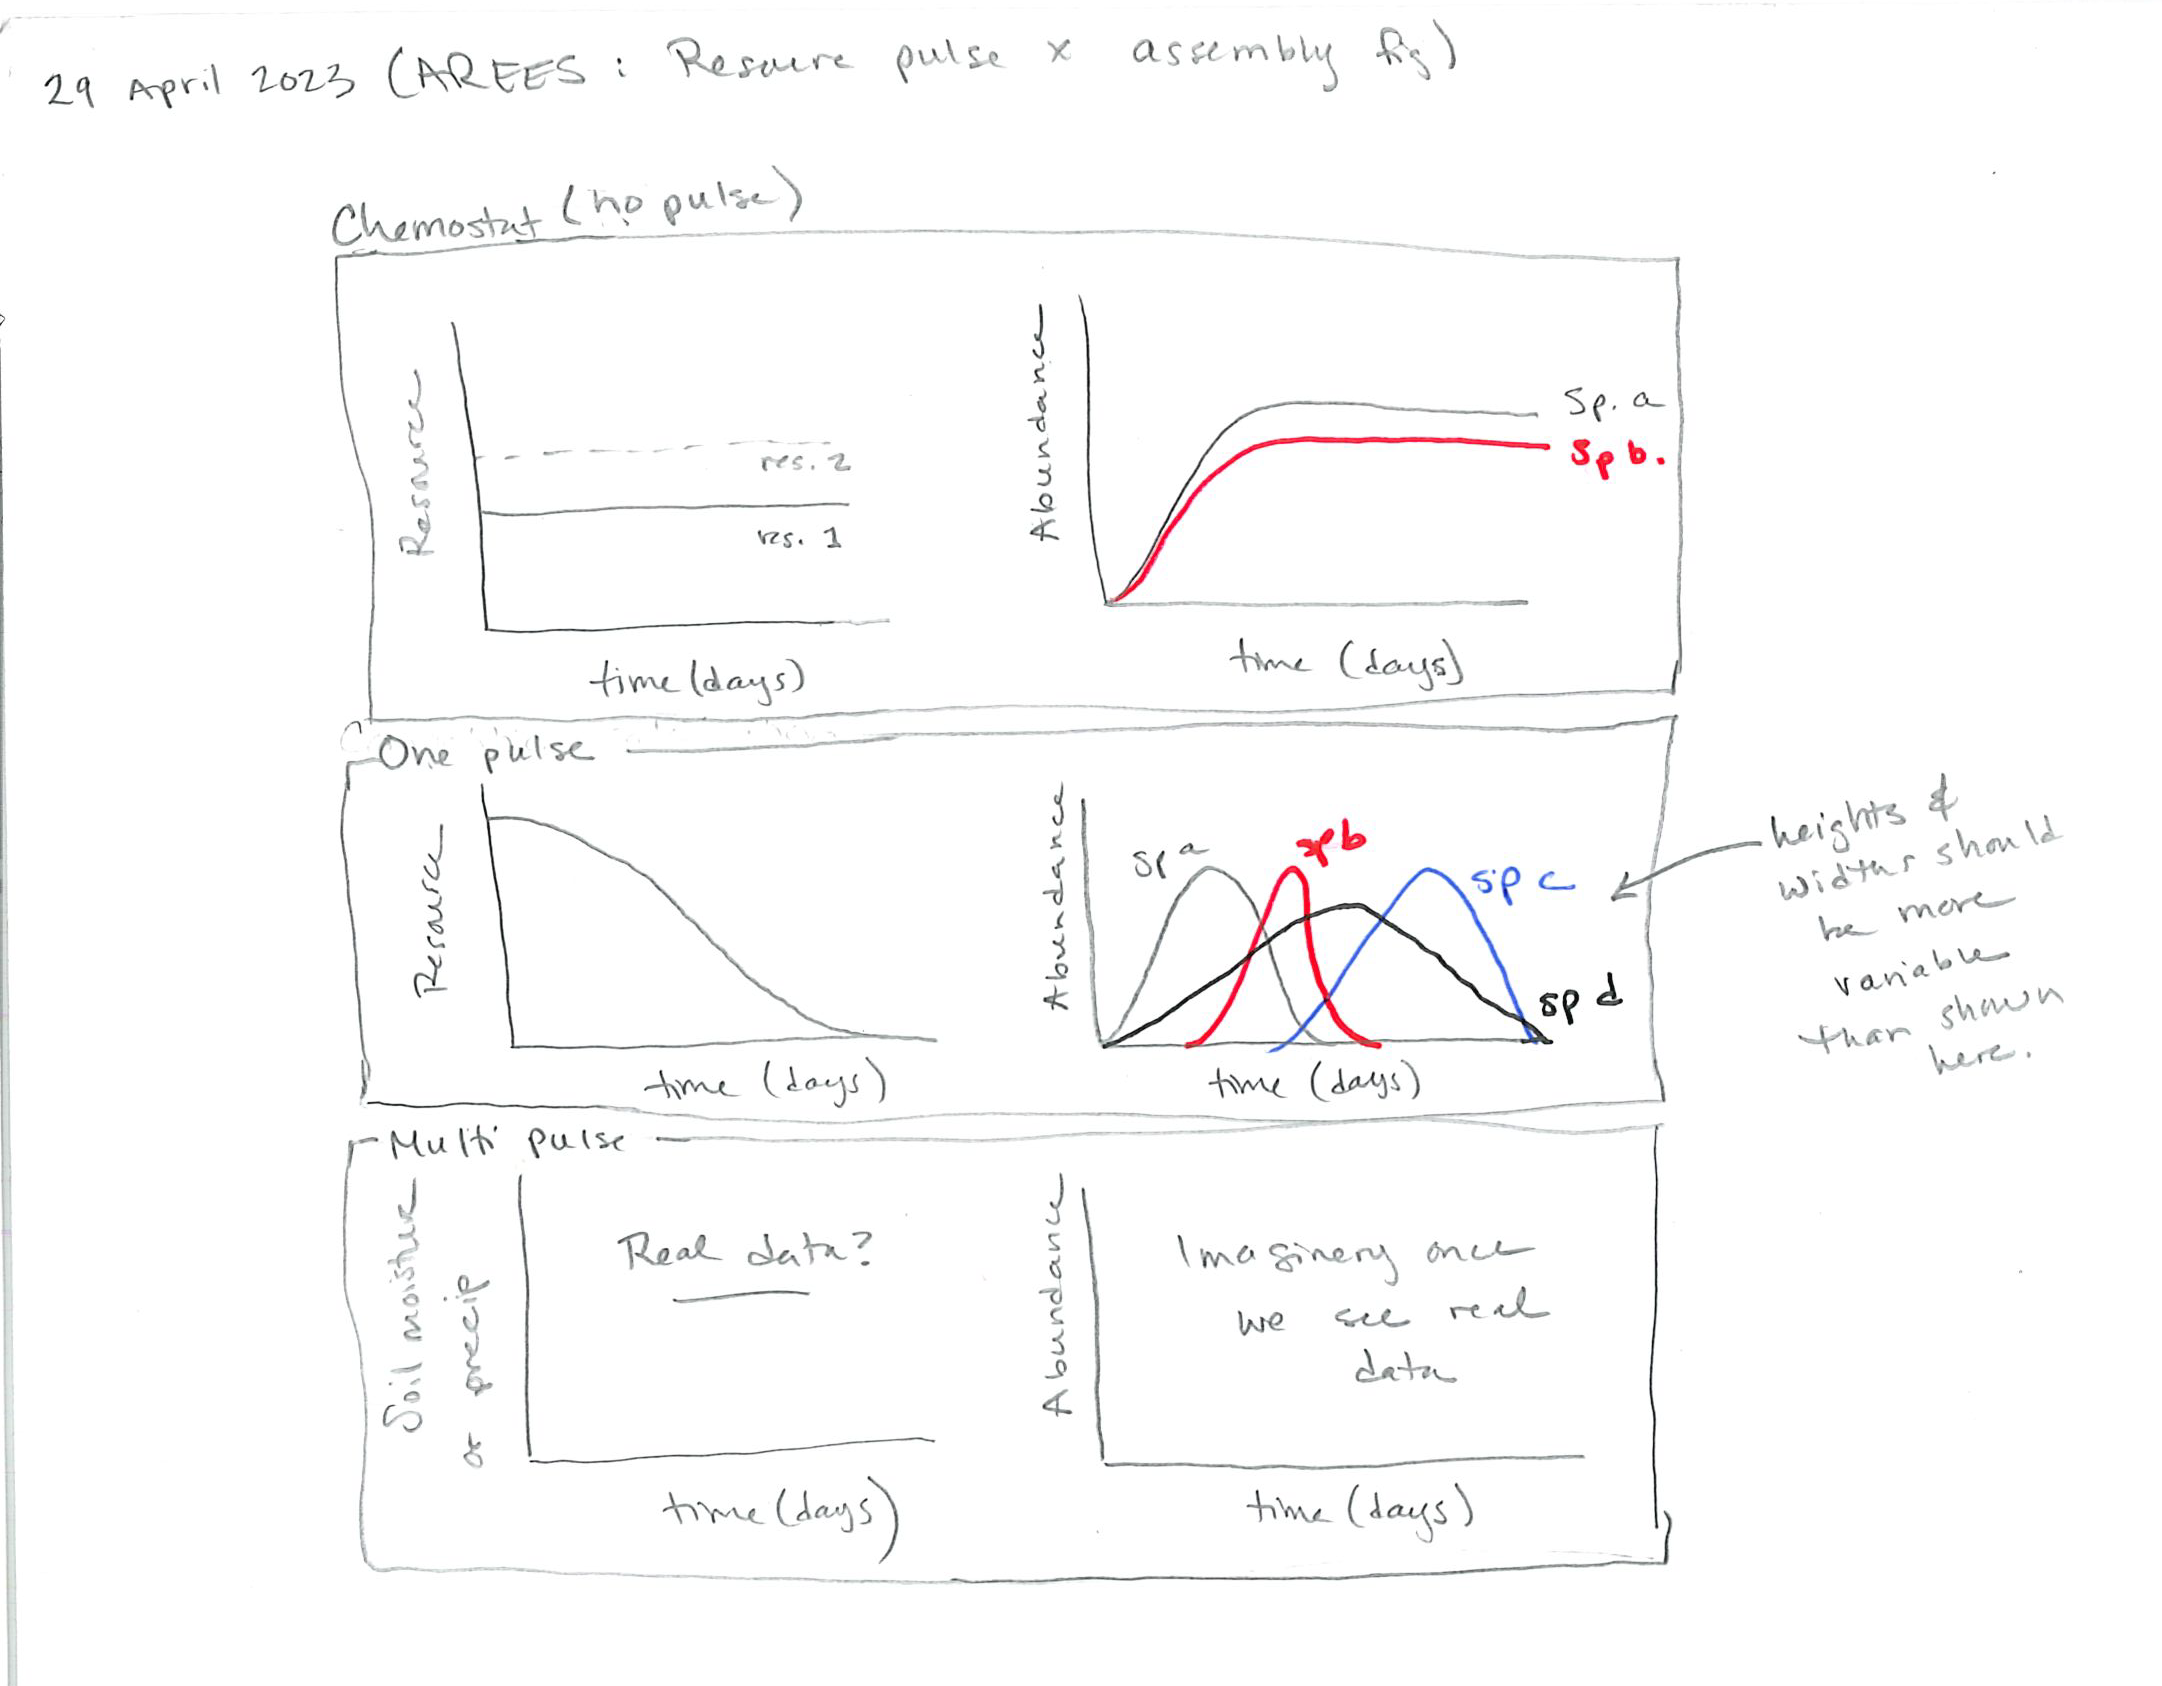
\includegraphics[width=1\textwidth]{..//figures/FigResourceApr2023.png}
\caption{Theory suggests resource levels may determine temporal niche space. In a system where resources are constant (top left,, chemostat; species can only coexist if they are each equally good competitors for different resources) species would be expected to show little temporal fluctuations. Many models of coexistence today, however, assume a resource pulse that decays (middle, left; e.g., water with evaporative loss) over time: this resource then sets the temporal window of each season and species compete within it. Most real systems however are more complicated (bottom left) ....}
 \label{fig:resource}
\end{figure}


\clearpage
\section{Miscellaneous meeting \& ref notes}

\emph{7 December 2023} Chat with Elsa.

May not be as predictive as we want, but we have so much evidence that phenology correlates with many traits -- but it's context dependent. 

Get friendly reviews from Deirdre, maybe Jonathan and Julie (Elsa's student).

\emph{24 November 2023: Black Friday} Chat with Elsa.

Refs from today or recently:

Phenological traits foster persistence of mutualistic networks by promoting facilitation (Duchenne et al. 2021) \url{https://onlinelibrary.wiley.com/doi/full/10.1111/ele.13836}

\emph{24 November 2023: Thinking about figures for life history x community ecology} 

Tried to track down any competitive related hypothesized trade-offs in life history and came up with ... 
\begin{enumerate}
\item Allocation of energy to .... growth/reproduction; growth/defense.
\item Size versus reproductive output
\item Maybe reproductive effort vs. competitive ability also? This would fit neatly into a phenology article. 
\item Early reproduction and lower competitive ability ($r$ selected species) Pianka 1970
\end{enumerate}

Colonization as more than just dispersal (so extends to budburst etc. perhaps): ``However, colonization is more than just dispersal because rapid population growth is also an important component of colonization." from Cadotte et al. 2006, `On Testing the Competition‐Colonization Trade‐Off in a Multispecies Assemblage' -- has a good figure I think (competition rank vs. colonization rank)

Trade-offs between stages matter. ``Finally, with respect to mechanisms promoting coexistence, we suggest that trade‐offs between different stages of colonization could be far more common in nature than a trade‐off between competitive ability and colonization ability." from Yu et al. 2001, `The Competition‐Colonization Trade‐off Is Dead; Long Live the Competition‐Colonization Trade‐off' (\url{https://www.journals.uchicago.edu/doi/abs/10.1086/320865})

\emph{30 October 2023} Chat with Elsa.

1) Phenology definitions ... I like the current one, other options:\\
a) the timing of critical stages of growth/reproduction and the transitions between them (new one that I am trying out)\\
b) timing of recurring growth and reproductive events (Ackerly pushed me to define it this way in a paper, but I am still unsure)\\

2) What to say about coexistence models, and how well they explain things ... if disturbance is more important than we think, then we may have early-species succeeding due to their colonization success ($r$-selected). 

3) What about predators/disease/etc? I can include some of this in the coexistence section. I should check on Fukami and disease. Also look for grass disease and phenology ... 

4) Trait optimum and coexistence -- species can only co-exist when both at the same trait optimum (see duckweed paper by Levine -- plasticity only contributes to coexistence when both are at the optimum)

5) Address plasticity -- non-plastic trait that appears plastic using calendar time... Say this somewhere. 

Misc) SKTmodel (1979)? `Spatial Segregation of Interacting Species'?
Maybe cite SKT model? Elsa has never heard of it, but maybe good to cite since so much Japanese lit get lost.

\emph{30 October 2023} Reviewing some references that I have been compiling ... 

{\bf I need to review!}

See also: Refs to work in above. 

Grainger, T.N., Letten, A.D., Gilbert, B. and Fukami, T., 2019. Applying modern coexistence theory to priority effects. Proceedings of the National Academy of Sciences, 116(13), pp.6205-6210. 

I should check on Fukami and disease. Also look for grass disease and phenology ... early-active individuals get hit (disease/predators is a little too hard to work on and a little too easy to ignore). 

{\bf Stuff on life history or related that I am excited about...} See also: Section 2 above. 

Cohen 1976 (of course), but more exciting! Iwasa \& Cohen 1989 (also maybe: Kubo \& Iwasa `Phenological Pattern of Tree Regeneration in a Model for Forest Species Diversity' -- not in my articles folder). 

Also check out Lyu \& Alexander and see below: Perrin \& Sibly 1993, King \& Roughgarden 1982, Yamamura (couple papers)

{\bf Probably have to cite}

Levine et al. 2022, `We modelled a system where all water arrives early in the season and species vary in their ability to grow under drying conditions. As a consequence, species differ in growing season length and compete by shortening the growing season of their competitors.'

Smith \& Amarasekare 2018: Intro says, `Differences between species in their responses to abiotic variation is a crucial prerequisite for coexistence via temporal niche partitioning.' 

Differences across range in phenology: Alexander et al. 2019 for potential invasive lettuce, Waterton et al. 2020, for two California grass species: `In both species, maternal lines with larger fractions of persistent seeds emerged later, indicating a trade-off between within-year emergence speed and potential among-year emergence spread.'

King \& Roughgarden 1982, `seed yield at time T may be maximized by a strategy consisting of two vegetative and two reproductive growth intervals under certain growth conditions.'

Perrin \& Sibly 1993 follows up on Cohen work:
\begin{quote}
This is illustrated in Figure 6a, for constant environment but variable season length. Here the norm of reaction is a monotonically decreasing function of age. In Cohen (16), production is proportional to vegetative biomass ($P = Ox$), and there is no mortality $(L = 0)$ so that Equation 13 reduces to $B(T - t) = 1$, which means that maturity
should occur at a fixed date before the season's end, independent of size. Indeed, Cohen (16) notes that late-flowering plants in cold temperate climates tend to flower at a fixed date. This corresponds to a vertical norm of reaction (Figure 6b).
\end{quote}

Yamamura et al. 2007: 

\begin{quote}
Some enclosure experiments have demonstrated that the onset of the peak flowering season is dependent on grazing pressure. We constructed a mathematical model using Pontryargin’s maximum principle to investigate changes in flowering time by examining shifts in resource allocation from vegetative to reproductive plant components. ... A higher herbivory rate on the vegetative components advanced the peak, whereas it was delayed when grazing pressure focused on reproductive components of the plant. In the non-linear production model, increased grazing pressure tended to postpone the flowering peak. These results corresponded well with results of enclosure experiments, thus suggesting adaptive control of flowering time in plants.
\end{quote}


Yamauchi \& Yamamura et al. 2004: Great overview of similar theory in intro:

\begin{quote}
Models ignoring life-history aspects seem applicable to simple organisms such as plankton, where the fitness of organisms can be measured by biomass. However, if we consider taxonomically higher plants, the model should include more detailed life history of the plants. In order to understand plant responses to herbivory, we should focus on the nutrient consumption pattern of plants, that is, the biomass allocation schedule or phenology. Among the studies that have considered evolution of the schedule of biomass allocation in plants, a mathematical approach that was initially developed by Cohen (1971, 1976) has played an important role. Thereafter, dynamic optimization models have successfully contributed to investigations on the evolution of plant phenology (King and Rough- garden 1982a, 1982b, 1983; Schaffer 1983; Iwasa and Roughgarden 1984; Iwasa and Cohen 1989; Iwasa 1991; Yamamura and Tsuji 1995; Iwasa et al. 1996; Iwasa and Kubo 1997). These studies have explained the resource allocation patterns between various tissues in a plant, which dynamically change during its life cycle.
\end{quote}

Kozlowski 1992 is a good review of the theory covered in Yamauchi \& Yamamura et al. 2004, including a discussion of how the switching is not as rapid as expected. Covers age and size at maturity a lot, which a lot of these papers cover... 

We say: Age and size at maturity---studied in annuals, but similar choices happen to a different degree (and with different consequences in long-lived individuals). 

Don't forget: Jops \& O'Dywer 2023; Ollerton \& Lack 1993

{\bf More articles}

Amarasekare 2020 is a good easy overview of Chesson's theory (Amarasekare 2000 is not so useful). \\
Armstrong \& McGehee 1980 -- classic on competitive exclusion. \\
Volaire papers, Vasseur paper, and Yamamichi et al. 2022 are less relevant. \\
Kikuzawa 1982, Kikuzawa 1995


\emph{17 October 2023} I chatted with Mark McPeek about coexistence theory (he has a new book!) and why coexistence theory and life history theory seem to predict the same results. On the latter he said, 'because people don't talk to each other.' On the former, he discussed how much competitive interactions dominate the field, when predators and other interactions matter so much. This point to me could be part of WHY coexistence theory and life history theory seem to converge---because community ecology is all about competition, which is a force that applies both within and between species (assuming life history is a lot about differences between individuals etc., when really it extends also to between species, but less so than community ecology if you ask me). 

He also sent a reference for a point he made, basically that there are some papers modifying competition models to cram in predators, which end up with needing negative predator pressure, effectively. I asked for a citation and replied:  

\begin{quote}
Chesson and Kuang cited in the coexistence book is the paper where they turn apparent competition into LV competition.  They don't make the point about the negative isoclines in their paper.  See Chapter 11 of the Coexistence book.

Also, here's a long unfinished draft of a manuscript on the topic.  I gotta get back to this one sometime.
\end{quote}

Look for `MacArthur Recasting' files. And in a follow-up reply he wrote:

\begin{quote}
You can find much of the discussion of the empirical studies in Chapter 11 of the book.  The paper develops a lot of stuff I didn't cover in the book.  But all the empirical studies are referenced there.
\end{quote}

\emph{5 July 2023} I chatted with Janneke and Jake Alexander about why life history and phenology seem to make the same predictions on the car ride home from Calanda. Janneke's take was that: they are related, perhaps by design with coexistence evolved from life history. But then why don't we teach it this way I asked? She said lots of fields are disconnected and end up doing their own little thing, ignoring other fields. Jake thought some of these general patterns extend across more than just life history and coexistence; for example this is basically R and K selection and that goes from population to community and also even (effectively) leaf economics spectrum. He also thought it could be historical and loaned me \emph{Modeling Nature} by Sharon E. Kingsland (1995, The University of Chicago Press, London (UK), 306 pp).

I later chatted with Jake Alexander about Lyu \& Alexander 2022, which seems relevant. Jake didn't have big insights for me on the coexistence space plot (told me not to focus too much on points or where they go) but I found the results interesting -- basically with competitors (interspecific density) most species trade-off vitals rates (but remember it's \emph{at a certain stage/size}). 

{\bf Side note:} Also might be worth mentioning the need to apply uncertainty to our parameterizations (see tables of numbers to third decimal place in `An expanded modern coexistence theory for empirical applications' by Ellner, for an example of what worries me). 

\emph{20 July 2023} chat with Jonathan Levine. To prep for this I went through his papers on coexistence and phenology and model on ISI (about 6 papers) and then a few recent refs:

\begin{itemize}
\item New paper: Integrating eco-evolutionary dynamics and modern coexistence theory (ELE) seems to get into the coexistence plots more and tries to interpret them. \url{https://onlinelibrary.wiley.com/doi/full/10.1111/ele.14078}
\item New Schreiber paper that seems super interesting and relevant! \url{https://esajournals.onlinelibrary.wiley.com/doi/full/10.1002/ecy.3838} Does deterministic coexistence theory matter in a finite world?
\item Should review more Alexander \& Levine 2019 PNAS: Earlier phenology of a nonnative plant increases impacts on native competitors
\item Jacob Levine phenology model ("We develop a general model of plants competing for water when soil water availability determines the duration of each competitor’s growing season") `Competition for water and species coexistence in phenologically structured annual plant communities'
\item{itemize}

Notes currently in gray notebook.

\end{document}

\begin{enumerate}
\item 
\end{enumerate}
